% Copyright (c) Jeff Smits
% This latex file is embedded in the pdf under license. 
% This license is called Creative Commons Attribution 3.0 Unported, 
% and is available at 
% http://creativecommons.org/licenses/by/3.0/legalcode or the LICENSE
% file in the git repository this tex file is in.

\documentclass[a4paper]{article}

\usepackage[english]{babel}

\usepackage{embedfile}
\embedfile[filespec=LaTeX-source]{\jobname.tex}
\embedfile[filespec=LICENSE]{LICENSE}

\usepackage{microtype}
\DisableLigatures[f]{encoding = *, family = *}

\usepackage{hyperref}
\hypersetup{
	pdftitle    = {Extreme Pong:\\
A browser-based game implemented using Functional Reactive Programming},
	pdfauthor   = {Jeff Smits},
	pdfkeywords = {UNITT} {UNITT 2012} {Pong} {Extreme Pong},
  colorlinks  = true,
  linkcolor   = black,
  citecolor   = black,
  filecolor   = black,
  urlcolor    = black
}

\usepackage{graphicx}

\begin{document}

\title{Extreme Pong: \\
A browser-based game implemented using Functional Reactive Programming}
\author{Jeff Smits}
\date{}

\maketitle

\begin{abstract}
Extreme Pong was created for the final round of the Universal IT Test (UNITT)
 2012. This is the accompanying document, which explains the structure of the
 game, what design decisions were made and why. 

Note that this document is under license ``Creative Commons
 Attribution 3.0 Unported''. The \LaTeX\ source is also available
 under the same license, it is attached to the PDF. 

\smallskip
\noindent\textbf{Keywords:} UNITT, UNITT 2012, Pong, Extreme Pong
\end{abstract}

\begin{figure}[h]
\centering
\setlength\fboxsep{0pt}
\setlength\fboxrule{1pt}
\fbox{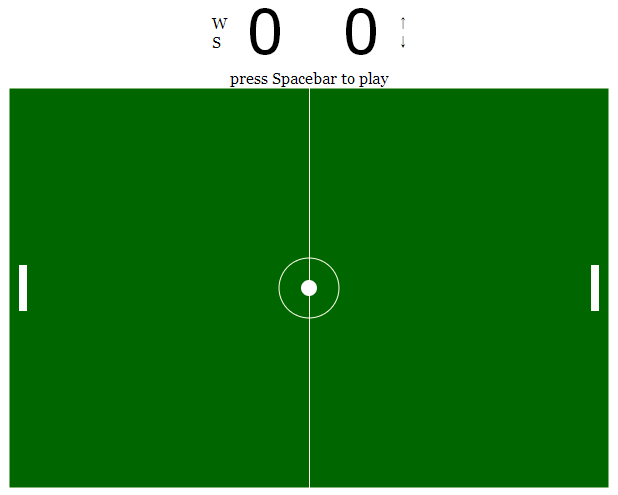
\includegraphics[width=\textwidth]{screenshot.png}}
\caption{A screenshot of the game. }
\label{fig:screenshot}
\end{figure}

\newpage

\section{Introduction}
Extreme Pong is a game which was designed with Pong as its base. The plan was to
 add features from Arkenoid, different maps with different shapes, some
 interesting physics... There was enough inspiration for an abundant list of
 features. 

The trouble was the way I personally wanted to program this game. I prefer
 functional programming. And not long ago I stumbled upon a language called Elm
 which seemed a perfect fit. It's a functional language that compiles to HTML,
 CSS and Javascript. So I jumped to the conclusion that this would be the
 perfect language. The problem with this language is that the project (and the
 compiler) are ten months old. And so I found out the language was far too young
 for developing anything with a deadline. But I had invested too much time in it
 already --- I only had seven days anyway --- so I stuck with it. 

This report will first explain a bit about Functional and Functional Reactive
 Programming. Then it will explain some of the problems I've experienced with
 learning and writing the Elm programming language. The report concludes with a
 review of the game, all its features, and a discussion of possible features.

\section{Functional Programming and FRP}

\subsection{Functional programming}
Imperative programming uses a composition of statements which change the global
 state. These statements instruct the computer \textit{how} to do something. \\
Functional programming uses expressions which model computations. It typically
 avoids mutable state. It is usually more about describing \textit{what} you
 want, rather than how you want the computer to do it. \footnote{This is a
 paraphrase of some text on the haskell wiki\cite{site:haskell-wiki-fp}}

Functional programming has a firm theoretical base in mathematics, and you can
 learn about it by learning about its theory. The lambda calculus would be the
 place to start, then perhaps some abstract algebra. I personally learnt a bit
 about it in a course during my first year as a Bachelor student in Computer
 Science. I then took the pragmatic approach and learnt a purely functional
 programming language. I can recommend the book ``Learn You a Haskell for Great
 Good'' \cite{book:LYaH}.

\subsection{Functional Reactive Programming (FRP)}
Functional Reactive Programming embraces the fact that values from the real
 world are variable, they change over time. In FRP these values are called
 \textit{signals}. Functions work on `normal' values which can be sampled from
 these signals, but this sampling is not programmed explicitly. Instead you
 lift these functions on top of a signal to produce another signal. This way you
 can sample, merge, create and transform signals. \footnote{I paraphrased some
 text from the Elm website here \cite{site:elm-frp}}

\section{Developing (issues) in Elm}
The Elm Programming Language brings Functional Programming to the web. To
 declaratively define GUIs, it uses Functional Reactive Programming. The
 language syntax is based on Haskell, but compiles to HTML and Javascript. 
 I already knew Haskell and Elm has an example program which implements a very
 simple version of Pong, so I thought this language was the perfect match for me
 and this project. 

Let me introduce you to some of the problems I've had with Elm 0.7.1.1.

\begin{enumerate}
\item Elm boasts an extensible record system which is supposed to be as powerful
 as typeclasses in Haskell. But they are not type-checked yet, and don't blend
 well with ADTs in my experience. 
\item The `multi-way if' is a nice language construct which generates
 strange compiler errors, so I don't use it. 
\end{enumerate}

Thankfully these language features are not paramount to writing programs in Elm.
 Some for the following problems really cripple the developement process though.
 
\begin{enumerate} \setcounter{enumi}{2}
\item Using modules to divide your program between multiple files is only
 allowed when you do not import the same file twice from two different
 locations. Because when your main module imports module 1 and module 2, and
 module 2 also imports module 1, this is perceived as a cyclic dependency. 
\item A function call to a function from a different module is not type-checked.
\item Type-checking generally misses some situations anyway, this results in
 run-time errors in Javascript. Sometimes these errors occur in the minified
 Elm run-time file, making it very hard to find out where in your program
 something went wrong.
\item When your Elm file gets larger and the functions get more complicated (and
 you can't use multiple files because of the cyclic dependency issue), the
 compiler takes longer and longer to compile you program. This is because the
 compiler has to infer the type of every function, which it has to do because
 type annotations are not yet supported. The longest compile time I've
 experienced was 45 minutes (no exaggeration, I timed it). 
\end{enumerate}

At some point, as more and more strange things happened --- some not listed
 because I couldn't keep count --- I decided to find help. Though Elm has some
 bugs in the compiler, the website is very clear and has a pretty complete
 documentation. It also has links to a webchat of their IRC channel, the github
 project where the compiler is developed open-source, and a mailing list.
 On the mailing list I found help from a very small but active and helpful
 community, and started using the developement version of the compiler. The
 benefit of this between-versions compiler is that it supports type annotations.

After finding some of the bugs from the above list and describing them on the
 mailing list, they were resolved very quickly by language creator Evan
 Czaplicki. I've looked into the compiler source code a number of times to find
 out if something was a compiler bug, and sometimes fixed the bug myself before
 reporting it.

\subsection{Concluding}
I wrote this section about my development problems in Elm to explain why I have
 created only a very simple game in the 7 days I had. \\
It is by no means meant as a discouragement to use Elm, but it might be
 advisable to use it for non-important projects. \\
It is also not meant as an excuse! I should have taken a better look at the
 language, or not use a new language on a project with a deadline. 

\section{The game of Extreme Pong}

The general structure of the game resembles the MVC model from imperative GUI
 programming. The difference is that using FRP makes it easy to keep the
 dependencies completely correct. An overview can be found in
 \autoref{fig:system-overview}. 

\begin{figure}[h]
\centering
\setlength\fboxsep{0pt}
\setlength\fboxrule{1pt}
\fbox{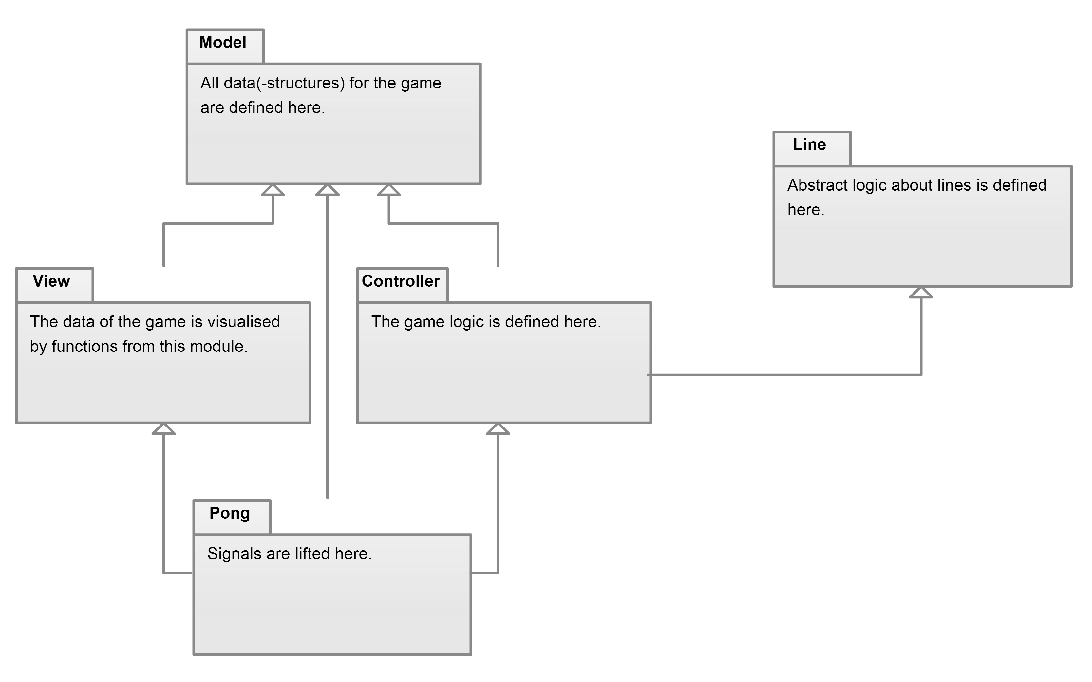
\includegraphics[width=\textwidth]{system-overview.pdf}}
\caption{A system overview of the game. }
\label{fig:system-overview}
\end{figure}

\subsection{Features}
Extreme Pong is the game of Pong with Arkenoid paddles. The visual features are:
\begin{itemize}
\item A rectangular field
\item Two paddles, one left and one right
\item A ball
\end{itemize}
The ball moves from the centre in a diagonal line. Both paddles can moves up and
 down using the keyboard. When the ball hits a field boundary it bounces off
 with the same angle as it hit the boundary. 

When the ball hits the paddle in the centre, the ball bounces off like in Pong.
 But the lower on the paddle the ball hits, the stronger the direction of the
 ball is influenced downward. The same idea higher on the paddle, the balls
 direction is changed upward. This features adds a bit of control to the game.
 This is what I call Arkenoid paddles. 

Apart from the different paddle behaviour, the difference between this game and
 the example game from the Elm website is that this version uses some math to
 calculate the trajectory of the ball when it hits something, in stead of
 reversing one of the axis of velocity of the ball when it has crossed the
 boundary of the field or a paddle. 

\subsection{Planned features}
A feature I had really planned to put into the game is \textbf{3+ player maps}.
 These maps would have a regular polygon shape to keep things interesting and
 easy for the implementation at the same time. The maximum amount of players
 would be equal to the amount of sides of the polygon, and less players would
 be able to play on polygon maps setting by unoccupied sides as field
 boundaries. 

Something else I had in mind for when I had time left was \textbf{gravitation
 points}. These would attract or repulse balls or paddles or both. A
 \textbf{slippery field} was another idea. The controls on the keyboard
 influence the paddle speed and there is be a low amount of friction. These
 two could also have been some sort of handicap that you could earn in the game.

\subsection{Performance}
On my computer, using the newest version of Google Chrome, the game performs at
 about 50 frame per second. 

\subsection{Future work}
I am thinking about continuing the development of this game. I still have
 plenty of ideas and plenty of things I want to try in Elm. I've also found
 an abstraction on collision that I want to develop so other Elm game
 developers can benefit from it as a library. 

\section{Conclusion}
By making this game I've learnt a new language and a new way to program GUIs. In
 this way I like to think of the project as time well spent. \\
But this game as the result of seven days\footnote{The arkenoid paddles were a
  last minute addition on the 8th day I worked on the game, but that was only an
  hour work extra} hard work is not much. And as a real project with a real
 deadline, I certainly did not perform as well as I could have. If I could do
 it all over, I would use Coffeescript as my implementation language with some
 Javascript libraries and some HTML and CSS.
 

\newpage

\bibliographystyle{plain}

\bibliography{report}

\end{document}